\sectioncentered*{Аннотация}
\thispagestyle{empty}

\begin{center}
  \begin{minipage}{0.82\textwidth}
    на дипломный проект <<Приложение для автоматизации процесса и поддержкибезопасной сдачи в аренду товаров для физических лиц>>
  \end{minipage}
\end{center}

Целью дипломного проекта является разработка приложение для автоматизации процесса и поддержкибезопасной сдачи в аренду товаров для физических лиц.
Во введении производится ознакомление с проблемой, решаемой в дипломном проекте.

В первой главе производится обзор предметной области проблемы решаемой в данном дипломном проекте.
Приводятся необходимые теоретические сведения, а также производится обзор существующих аналогов.
ФОрмулируются требования к программному обеспечени.

Во второй главе производится краткий обзор технологий, использованных для реализации ПО в рамках дипломного проекта.

В третьей главе производится проектирование ПО.
Описываются его составные части и особенности.

В пятой главе производится описание разработкри ПО.
Описывается разработка серверной и клиентской части приоложения.
Описывается контейнеризация приложения в Docker.

В шестой главе производится технико"=экономическое обоснование разработки.

В заключении подводятся итоги и делаются выводы по дипломному проекту, а также описывается дальнейший план развития проекта.

Дипломный проект выполнен самостоятельно и проверен в системе «Антиплагиат».
Процент оригинальности соответствует норме, установленной кафедрой информатики.
Цитирования обозначены ссылками на публикации, указанные в «Списке литературы».

\begin{figure}[h]
  \centering
  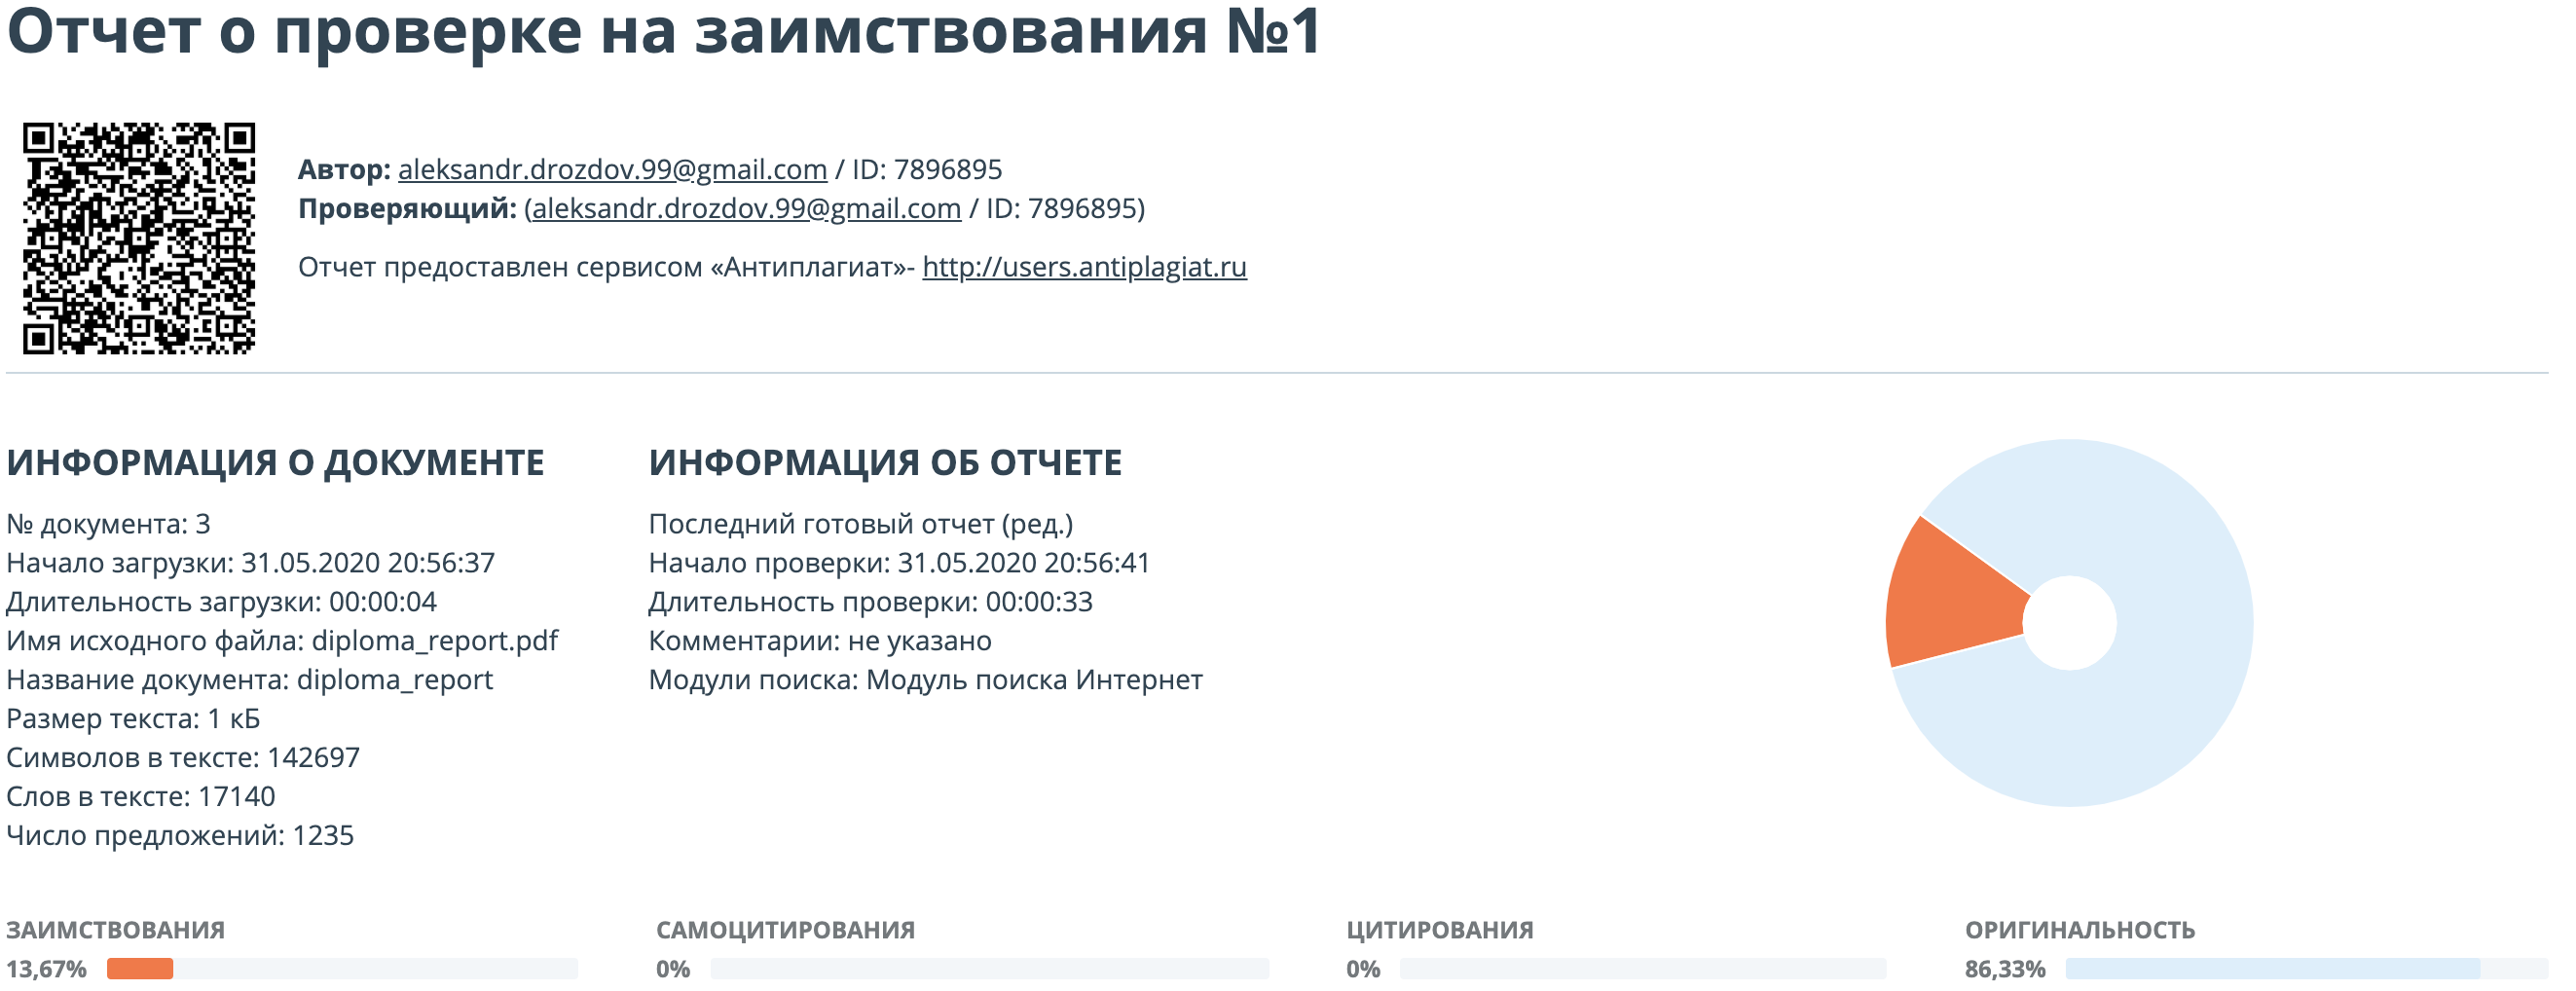
\includegraphics[scale=0.3]{antiplagiat.png}
\end{figure}

\clearpage
